\documentclass[12pt]{article}
\usepackage{ctex}
\usepackage[english]{babel}
\usepackage{blindtext}
\usepackage{nameref}
\usepackage{fancyhdr}
\usepackage{amsmath,amssymb,amsthm}
\usepackage{graphicx,float}
\usepackage{physics}
\usepackage{pgfplots}
\usepackage[a4paper, total={7in, 9in}]{geometry}

\graphicspath{{./img/}}

\pagestyle{fancy}
\fancyhf{}
\fancyhf[HL]{測驗1:二項式定理、指數及對數}
\fancyhf[CF]{\thepage}

\newcommand{\innerprod}[2]{\langle{#1},{#2}\rangle}
\newcommand{\id}{\mathtt{id}}

\newtheorem{definition}{定義}
\newtheorem*{theorem}{定理}
\newtheorem*{corollary}{衍理}
\newtheorem*{lemma}{引理}
\newtheorem*{proposition}{設理}
\newtheorem*{remark}{小記}
\newtheorem*{claim}{主張}
\newtheorem*{example}{例子}
\newtheorem*{axiom}{公設}
\renewenvironment*{proof}{\textit{證明.}}{\hfill$\qed$}

\newenvironment*{sol}{\par \textbf{解}.}{\hfill$\blacksquare$}

\begin{document}
    \begin{enumerate}
        \item \begin{enumerate}
            \item \begin{flalign*}
                \biggl(u+\frac{1}{u}\biggr)^4&=u^4+4u^3\biggl(\frac{1}{u}\biggr)+6u^2\biggl(\frac{1}{u}\biggr)^2+4u\biggl(\frac{1}{u}\biggr)^3+\biggl(\frac{1}{u}\biggr)^4\\
                &=u^4+4u^2+6+\frac{4}{u^2}+\frac{1}{u^4}
            \end{flalign*}
            \item \begin{flalign*}
                (e^{ax}+e^{-ax})^4&=e^{4ax}+4e^{2ax}+6+4e^{-2ax}+e^{-4ax}\\
                &=\biggl[1+\frac{4ax}{1!}+\frac{(4ax)^2}{2!}+\cdots\biggr]+4\biggl[1+\frac{2ax}{1!}+\frac{(2ax)^2}{2!}+\cdots\biggr]+6\\&+4\biggl[1+\frac{-2ax}{1!}+\frac{(-2ax)^2}{2!}+\cdots\biggr]+\biggl[1+\frac{-4ax}{1!}+\frac{(-4ax)^2}{2!}+\cdots\biggr]\\
                &=1+4ax+8a^2x^2+4+8ax+8a^2x^2+6\\&+4-8ax+8a^2x^2+1-4ax+8a^2x^2+\cdots\\
                &=16+32a^2x^2+\cdots
            \end{flalign*}
            \item \begin{flalign*}
                32a^2&=2\\
                a^2&=\frac{1}{16}\\
                a&=\pm\frac{1}{4}
            \end{flalign*}
        \end{enumerate}
        \item \begin{flalign*}
            (1+e^{3x})^2&=1+2e^{3x}+e^{6x}\\
            &=1+2\biggl[1+\frac{3ax}{1!}+\frac{(3ax)^2}{2!}+\cdots\biggr]+\biggl[1+\frac{6ax}{1!}+\frac{(6ax)^2}{2!}+\cdots\biggr]\\
            &=4+12x+27x^2+\cdots
        \end{flalign*}
        \item \begin{flalign*}
            (5-x)^4&=5^4-C_1^4(5^3)x+C_2^4(5^2)x^2+C_3^4(5)x^3+x^4\\
            &=625-500x+150x^2-20x^3+x^4
        \end{flalign*}
        所求係數:\begin{flalign*}
            &=(625)(27)+(-500)(12)+(150)(4)\\
            &=11475
        \end{flalign*}
        \item\begin{enumerate}
            \item \begin{flalign*}
                N(t)&=\frac{500}{1+ae^{-kt}}\\
                \ln\biggl(\frac{500}{N(t)}-1\biggr)&=\ln(ae^{-kt})\\
                &=-kt+\ln{a}
            \end{flalign*}
            \item 先求所需數值:\begin{center}
                \begin{tabular}{|c|c|c|c|c|}
                    \hline
                    $t$&5&10&15&20\\
                    \hline
                    $\ln\biggl(\frac{500}{N(t)}-1\biggr)$&3.6&2.6&1.6&0.6\\
                    \hline
                \end{tabular}
            \end{center}
            圖像如下:
            \begin{figure}[H]
                \centering
                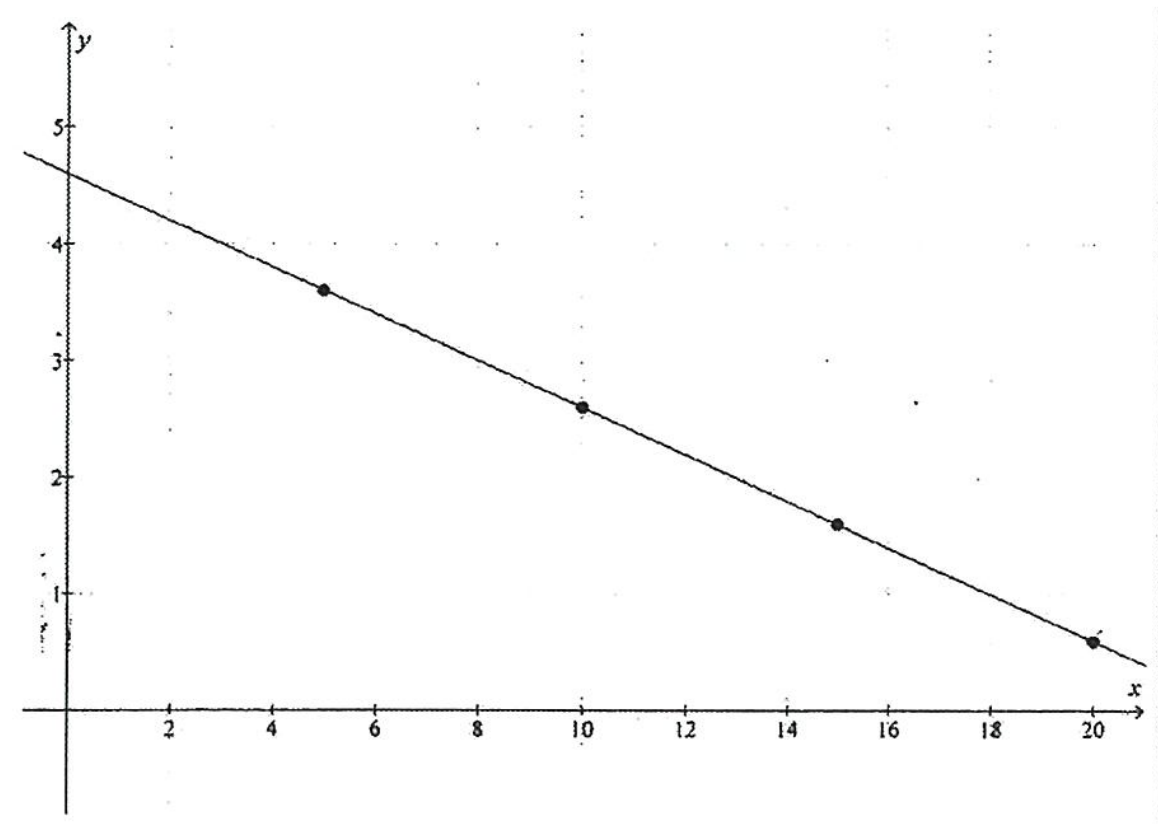
\includegraphics[scale=0.8]{graph_sol.png}
            \end{figure}
            從圖像可得
            \begin{flalign*}
                \ln{a}&\approx 4.6\\
                a&\approx 99.48431564\\
                &\approx 99.5\\
                -k&=\frac{0.6-3.6}{20-5}\\
                k&=0.2
            \end{flalign*}
            \item \begin{flalign*}
                270&=\frac{500}{1+99.48431564e^{-0.2t}}\\
                t&=23.80171325
            \end{flalign*}
            因此,疾病爆發後的第24天,受感染的魚的數量會到達270條。
        \end{enumerate}
        \item[挑戰題.]\begin{enumerate}
            \item \begin{flalign*}
                \sum_{k=0}^{n}a_k&=\sum_{k=0}^{n}C_k^n p^k(1-p)^{n-k}\\
                &=(1-p+p)^n\\
                &=1
            \end{flalign*}
            \item \begin{flalign*}
                k\cdot C_k^n&=k\cdot\frac{n!}{k!(n-k)!}\\
                &=k\cdot\frac{n(n-1)!}{k(k-1)!(n-k)!}\\
                &=n\cdot\frac{(n-1)!}{(k-1)!(n-k)!}\\
                &=n\cdot\frac{(n-1)!}{(k-1)![(n-1)-(k-1)]!}\\
                &=n\cdot C_{k-1}^{n-1}
            \end{flalign*}
            \begin{flalign*}
                \sum_{k=0}^{n}ka_k&=\sum_{k=1}^{n}k\cdot C_k^{n}p^k(1-p)^{n-k}\\
                &=\sum_{k=1}^{n}n\cdot C_{k-1}^{n-1}p^k(1-p)^{n-k}\\
                &=n\sum_{k=0}^{n-1}\cdot C_{k}^{n-1}p^{k+1}(1-p)^{n-k-1}\\
                &=np\sum_{k=0}^{n-1}\cdot C_{k}^{n-1}p^{k}(1-p)^{n-k-1}\\
                &=np(1)\\
                &=np
            \end{flalign*}
        \end{enumerate}
    \end{enumerate}
\end{document}